\documentclass[a4paper, 12pt]{article}

\usepackage{geometry}
\usepackage{textcomp}					% "true" символы типа copyright

\usepackage{cmap}						% Улучшенный поиск русских слов в полученном pdf-файле
\usepackage[T2A]{fontenc}				% Поддержка русских букв
\usepackage[utf8]{inputenc}				% Кодировка utf8
\usepackage[english, russian]{babel}	% Языки: русский, английский
\usepackage[unicode]{hyperref}			% Русский язык для оглавления pdf
\usepackage{bookmark}					% Оглавление в pdf
\usepackage{soulutf8}					% Для разрядки

\usepackage{amssymb,amsmath,amsthm}
\usepackage{graphicx} 					% Подключаем пакет работы с графикой
\usepackage[ruled]{algorithm}
\usepackage[noend]{algpseudocode}

\usepackage{color}

\usepackage{titlesec}					% Форматирование заголовков
%\usepackage{abstract}					% Форматрирование абстракта	

\geometry{a4paper,top=2cm,bottom=2cm,left=2.5cm,right=1cm}	% Геомтерия страницы
\graphicspath{{../../images/}} 			% Пути к изображениям

%\renewcommand{\baselinestretch}{2}

% Настройка теоремоподобных окружений
\theoremstyle{plain}
\newtheorem{Theorem}{Теорема}
\newtheorem{Lemma}[Theorem]{Лемма}
\newtheorem{Pred}{Утверждение}
\newtheorem{Corollary}{Следствие}
\newtheorem{Def}{Определение}
\newenvironment{Proof}%
	{\par\noindent{\bf Доказательство.}}%
	{\hfill$\scriptstyle\blacksquare$}

\floatname{algorithm}{}
\newcommand{\algrule}[1][.2pt]{\par\vskip.2\baselineskip\hrule height #1\par\vskip.2\baselineskip}
\algrenewcommand\algorithmicrequire{\textbf{Вход:}}
\algrenewcommand\algorithmicensure{\textbf{Выход:}}
\algrenewcommand\algorithmicforall{\textbf{для всех}}
\algrenewcommand\algorithmicwhile{\textbf{пока}}
\algrenewcommand\algorithmicif{\textbf{если}}
\algrenewcommand\algorithmicthen{\textbf{то}}
\algrenewcommand\algorithmicelse{\textbf{иначе}}
\algrenewcommand\algorithmicreturn{\textbf{вернуть}}
\algrenewcommand\algorithmicfunction{\textbf{процедура}}
\algrenewcommand\algorithmicdo{}
\renewcommand{\algorithmiccomment}[1]{{\quad\sl // #1}}

\renewcommand\labelenumi{\theenumi )}	% Нумерованный перечень со скобками
\AtBeginDocument{\renewcommand{\abstractname}{\vspace{-2\baselineskip}}}    		% clear the title
%\renewcommand{\absnamepos}{empty} % originally center

\makeatletter
	\bibliographystyle{gost2008p}
	\renewcommand{\@biblabel}[1]{#1.}	% Заменяем библиографию с квадратных скобок на точку:
\makeatother

\titleformat{\section}[runin]{\normalfont\bfseries}{\thesection.}{1pt}{}[.]
\titleformat{\subsection}[runin]{\normalfont}{\thesubsection.}{1pt}{\so}[.]
%\titleformat{command}[shape]{format}			   {label}		 {sep}{before}[after]

\DeclareMathOperator*{\argmax}{arg\,max}
\DeclareMathOperator*{\argmin}{arg\,min}

\title{\hbox{\normalsize\textit{УДК 004.81}}\hbox{}\textbf{\Large\MakeUppercase{Управление поведением как функция сознания. II. Самосознание и синтез плана}}\footnote{Работа выполнена при поддержке РНФ (грант \No\ 14-11-00692).}}
\author{\textbf{\textcopyright~2015~г. Г.\,С.~Осипов, А.\,И.~Панов, Н.\,В.~Чудова}\\\normalsize\textit{Москва, Институт системного анализа РАН}}
\date{}

\begin{document}
	\vspace*{-5\baselineskip}			% Убираем лишние пробелы перед заголовком статьи
	{\let\newpage\relax\maketitle}
	
	\begin{abstract}
		\noindent Рассматриваются описания функций, которые в психологии принято относить к функциям сознания и самосознания. Анализируется взаимодействие компонент знака, введённых в первой части статьи, исследуется сходимость основного итерационного процесса образования пары образ "--- значение. Строится алгоритм синтеза плана поведения и предлагается новая архитектура интеллектуальных агентов, обладающих, в частности, способностями к распределению ролей в коалициях.
	\end{abstract}	
	
	\section*{Введение}
	В первой части настоящей работы \cite{PanovA2014a},рассмотрена модель знака, как основной компоненты картины мира субъекта деятельности. Предложены основные процедуры формирования знака. Исследованы процессы самоорганизации на множестве знаков, благодаря которым оказывается возможным описать различные типы картин мира субъектов деятельности.
	
	В основе нашего рассмотрения лежат идеи культурно-исторического подхода Выготского"--~Лурии \cite{Luria1970,Vygotsky2005}, теория деятельности Леонтьева \cite{Leontiev1975} и модель психики Артемьевой \cite{Artemyeva1980}. Согласно приведённым теориям высшие когнитивные функции реализуются в рамках мотивированной предметной деятельности, когда объекты и процессы внешней  среды опосредованы для субъекта специальными образованиями, называемыми знаками. Благодаря наличию четырёх компонент: образа, значения, личностного смысла и имени "--- знак участвует в реализации тех или иных когнитивных функций. 
	
	Четырёхкомпонентная структура элемента индивидуального знания, которая, как было сказано выше, в психологии называется знаком, подтверждается и теми работами нейрофизиологов, в которых предпринимается попытка построить общую теорию работы мозга человека. Так, в теории повторного входа Эделмена \cite{Edelmen1981} и гипотезе информационного синтеза Иваницкого \cite{Ivanitsky1996,Ivanitsky2010} утверждается, что возникновение ощущения или осознанная фиксация входного потока информации происходит только в том случае, когда активированное сенсорным входом возбуждение от гиппокампа, а затем от гипоталамуса, накладывается на сенсорный след в проекционной коре. Такой <<круг ощущений>> (рис. \ref{fig:ivan_cyrcle}), проходящий за характерное время в 150-300 мс, последовательно активирует три компоненты индивидуального знания: образную (проекционная и сенсорная зоны коры), компоненту значения (гиппокамп) и личностного смысла (гипоталамус). Регистрация сигнала в лобных долях (после возврата его в зоны первичной проекции), по видимому, связана с именованием всех трёх активированных компонент.
	
	\begin{figure}[h]
		\centering
		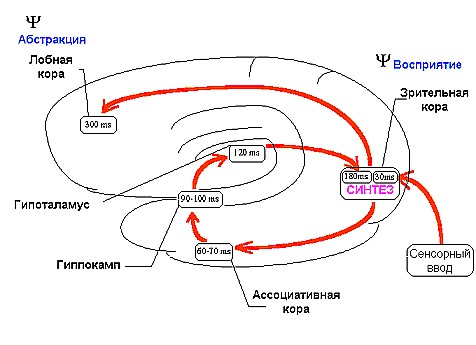
\includegraphics[width=0.7\linewidth]{ivanitsky_cyrcle}
		\caption{<<Круг ощущений>> по Иваницкому \cite{Ivanitsky1996}.}
		\label{fig:ivan_cyrcle}
	\end{figure}
	
	Кроме того, по современным нейрофизиологическим представлениям строение коры головного мозга практически однородно во всём своём объёме, о чём свидетельствует наличие макро- и миниколонок неокортекса \cite{Mountcastle1998,Rockland2010}. При этом связи между достаточно малыми зонами коры (так называемый коннектом \cite{Zador2012}), явно указывают на иерархичность её строения и на присутствие как восходящих, так и обратных, нисходящих связей. Отсюда следует, что основные компоненты элемента индивидуального знания должны обладать иерархическим однородным строением с восходящими потоками информации и нисходящей обратной связью. Кроме того, образная компонента должна иметь такую функцию распознавания, которая кроме категоризации процессов и статических объектов использует обратную связь для предсказания сигнала в следующий момент времени.
	
	\section{Модельный (или семантический) уровень}
	В качестве модели базовой составляющей основных компонент знака будем использовать специальный распознающий автомат ($R$-автомат) $R=<A,Q,B,\varphi, \eta>$, где $A$ "--- множество входных сигналов, $B$ "--- множество выходных сигналов, $Q$ "--- множество состояний, $\varphi$ "--- функция переходов, $\eta$ "--- функция выходов. Входные и выходные сигналы будем задавать с помощью множества признаков $\mathcal F$. Основными функциями распознающего автомата являются следующие:
	\begin{itemize}
		\item хранение информации о множестве некоторых сходных явлений (предметов и процессов внешнего мира), которые будем называть множеством выходных признаков $F^*\in\mathcal F$ этого автомата,
		\item распознавание выходных признаков из множества $F^*$ по информации о входных признаках из множества $F\in\mathcal F,F\cap F^*=\varnothing$, с помощью функций распознавания из множества $\hat F$.
	\end{itemize}
	
	Действие функции распознавания заключается в сопоставлении каждому признаку $f_k$ из множества $F^*$ действительного значения $x_k^*$, вычисляемого по входному вектору $\bar x$. Значение $x_k^*$ определяет уровень доверия тому, насколько успешно удалось построить признак из составляющих его низкоуровневых признаков, взвешенные значения присутствия которых во входном сигнале определяются вектором $\bar x$. В этом случае будем говорить, что распознающий автомат $R$ распознает признак $f_k$: $f_k\dashv R$.
	
	В соответствии с данными нейрофизиологов будем считать, что множество $R$-автоматов $\mathcal R$ организовано в иерархическую схему в виде связного ориентированного ярусного графа. Выход распознающего автомата $R_i^j=<A_i^j,Q_i^j,B_i^j,\varphi_i^j, \eta_i^j>, R_i^j\in\mathcal R$, направляется на следующий уровень иерархии; на вход поступает, соответственно, сигнал с предыдущего уровня. Нижний индекс распознающего автомата является сквозным по множеству $\mathcal R$, а верхний обозначает номер яруса, которому принадлежит автомат.
		
	Опишем подробнее множества выходных и выходных сигналов распознающего автомата, а также его множество состояний.
	
	Входом $R$-автомата является множество пар векторов $(\bar x,\hat x^{j+1})$, где первый вектор пары является вектором размерности $q$ весов входных признаков, а второй "--- управляющим вектором размерности $l$ со следующего уровня иерархии, который принимает ненулевое значение только в фиксированные для данного автомата моменты времени $0,h,2h,\dots$. Таким образом, множество входных сигналов $A$ является декартовым произведением пространств взвешенных векторов входных признаков $X$ и управляющих векторов со следующего уровня иерархии $\hat X^{j+1}$: $A=X\times \hat X^{j+1}$. 
	
	Выходом $R$-автомата является множество пар $(\bar x^*,\hat x^j)$, где $\bar x^*$ "--- это вектор весов выходных признаков размерности $l$, а $\hat x^j$ "--- управляющий вектор размерности $q$ для предшествующего уровня иерархии, который наряду с выходами других автоматов уровня $j$ является входным управляющим вектором для некоторых автоматов уровня $j-1$. Из этого следует, что за единицу времени для автоматов уровня $j$ проходит $h^{j-1}$ единиц времени для автоматов уровня $j-1$. Таким образом, выходное множество $B$ является декартовым произведением пространств взвешенных векторов выходных признаков $X^*$ и управляющих векторов для предшествующего уровня иерархии $\hat X^j$: $A=X^*\times \hat X^j$.
	
	Будем считать множество состояний конечным, в связи с чем каждой функции распознавания $\hat f_k$ из множества $\hat F$ будем ставить в соответствие набор матриц предсказания $Z_k=\{Z_1^k,…,Z_m^k\}$ размерности $q\times h$, где $h$ "--- характерное время распознающего автомата. Столбец $\bar{z}_u^r=(z_{u1}^k,…,z_{uq}^k)$ матрицы $Z_r^k$ интерпретируется как вектор предсказания присутствия входных признаков из множества $F$ в момент времени $\tau+u$, где $\tau = 0,h,2h,\dots$. При этом $z_{uv}^k\in\{0,1\}$, т.~е. вектор $\bar{z}_u^r$ является булевым вектором. Сама матрица $Z_r^k$ задаёт, таким образом, последовательность событий, наличие которых свидетельствует о~присутствии распознаваемого функцией $\hat f_k$ признака. Иными словами, множество всех матриц предсказания распознающего автомата $\mathcal Z$ хранит в себе информацию о выходных признаках. Множество состояний будем определять как совокупность всех подмножеств множества всех матриц предсказания: $Q=2^{\mathcal Z}$.
	
	Алгоритм $\mathcal A_{th}$ вычисления функции переходов $\varphi:X\times\hat X^{j+1}\to 2^{\mathcal Z}$ и выходной функции $\eta:2^{\mathcal Z}\to X^*\times\hat X$ по начальному моменту времени $\tau$, управляющему воздействию $\hat x^{j+1}(\tau)$ и входному воздействию $\omega:T\to X$ представлен ниже. В алгоритме используется стандартная функция $W$ нормировки весовых значений:
	\begin{equation}
	W(\bar x)=\left(\frac{x_1}{\max\limits_i x_i},\dots,\frac{x_n}{\max\limits_i x_i}\right),
	\end{equation} 
	где $\bar x=(x_1,\dots,x_n)$ "--- вектор с ненормированными компонентами.
	
	В следствие особенностей алгоритма $\mathcal A_{th}$ и  того, что множества входных и выходных сигналов являются векторными пространствами, распознающий автомат $R$ является бесконечным автоматом Мили с переменной структурой и конечной памятью (рис. \ref{fig:rb_io}): 
	\begin{equation}
	R_i^j=<X\times\hat X^{j+1}, 2^{\mathcal Z}, X^*\times\hat X^j,\varphi_i^j,\eta>.
	\end{equation}

	\begin{algorithm}
		\caption{Алгоритм $\mathfrak{A}_{th}$ вычисления автоматной функции распознающего автомата $R_i^j$}\label{alg:automato}
		\begin{algorithmic}[1]
					\Require $\tau_s, \hat{x}_i^{j+1}(\tau_s), \omega_i^j$.
		\Ensure $\varphi_{i\Delta t}^j, \vec\eta_{i\Delta t}^j$.

		\State $\hat{F}^*=\varnothing,Z^*=\varnothing,t=0$; \Comment{активные функции распознавнаия и матрицы предсказания}
		\State $c_1\in(0,1), c_2\in(0,1)$; \Comment{пороговые константы}

		\Statex \Comment{определение начального состояния}
				
		\ForAll{компонент $\hat{x}_{ik}^{j+1}$ вектора $\hat{x}_i^{j+1}(\tau_s)=(\hat{x}_{i1}^{j+1},\hat{x}_{i2}^{j+1},\dots,\hat{x}_{il}^{j+1})$} \label{alst:init_start}
			\If{$\hat{x}_{ik}^{j+1}{\ge}c_1$} \label{alst:select_f}
				\State $\hat{F}^*:=\hat{F}^*\cup\{\hat{f}_k\}$;
			\EndIf
		\EndFor
		
		\State $\bar x_i^j:=\omega_i^j(\tau_s)$;
		
		\ForAll{функций распознавания $\hat{f}_k\in\hat{F}^*$}
			\ForAll{$Z_r^k\in Z_k$, соответствующих функции распознавания $\hat{f}_k$,}
				\If{$\frac{\|\bar{z}_1^r-\bar{x}_i^j\|}{\|\bar{z}_1^r\|+\|\bar{x}_i^j\|}<c_2$} \label{alst:select_z}
					\State $Z^*:=Z^*\cup\{Z_r^k\}$;
				\EndIf
			\EndFor
		\EndFor
		
		\State $\varphi_i^j(\bar x_i^j,\hat{x}_i^{j+1}(\tau_s)) := Z^*$; \Comment{значение функции переходов в начальный момент времени}\label{alst:init_state}
		\State $\bar N:=(|\{Z_r^1|Z_r^1\in Z^*\}|,\dots,|\{Z_r^{l_i^j}|Z_r^{l_i^j}\in Z^*\}|)$; \label{alst:init_calc_out2}
		\State $\eta(Z^*)=\bar{x}_i^{*j}:=W(\bar N)$; \Comment{значение функции выходов в начальный момент времени} \label{alst:init_calc_out3}
		\State $\hat x_i^j=W(\sum_{\hat f_k\in\hat F^*}\hat x_{ik}^{j+1}\sum_{Z_r^k\in Z^*}\bar z_2^r)$;\label{alst:init_control}
		\label{alst:init_end}
				\Statex \Comment{основной цикл}
	
	\State $t=1$;
	\While{$t\leqslant{h_i^j}-1$} \label{alst:cycle_start}
		\State $\bar{x}_i^j:=\omega(\tau_s+t)$;
	
		\ForAll{матриц предсказания $Z_r^k$ из множества $Z^*$}
			\If{$\frac{\|\bar{z}_{t+1}^r-\bar{x}_i^j\|}{\|\bar{z}_{t+1}^r\|+\|\bar{x}_i^j\|}\geqslant{c_2}$} \label{alst:update_z}
				\State $Z^*:=Z^*\setminus\{Z_r^k\}$;
			\EndIf
		\EndFor
	
		\State $\varphi_i^j(\bar x_i^j,\hat{x}_i^{j+1}(\tau_s)) := Z^*$; \Comment{значение функции переходов в момент времени $t$}
		\State $\bar N=(|\{Z_r^1|Z_r^1\in Z^*\}|,\dots,|\{Z_r^{l_i^j}|Z_r^{l_i^j}\in Z^*\}|)$; \label{alst:calc_out1}
		\State $\eta(Z^*)=\bar{x}_i^{*j}:=W(\bar N)$;\Comment{значение функции выходов в момент времени $t$} \label{alst:calc_out3}
	
		\State $t=t+1$;
		\If{$t\leqslant{h}_i^j-2$}
			\State $\hat{x}_i^j:=W(\sum_{\hat f_k\in\hat F^*}\hat x_{ik}^{j+1}\sum_{Z_r^k\in Z^*}\bar z_t^r)$; \label{alst:calc_state1}
		\EndIf
	\EndWhile \label{alst:cycle_end}
		\end{algorithmic}
	\end{algorithm}
	
	\begin{figure}[H]
		\centering
		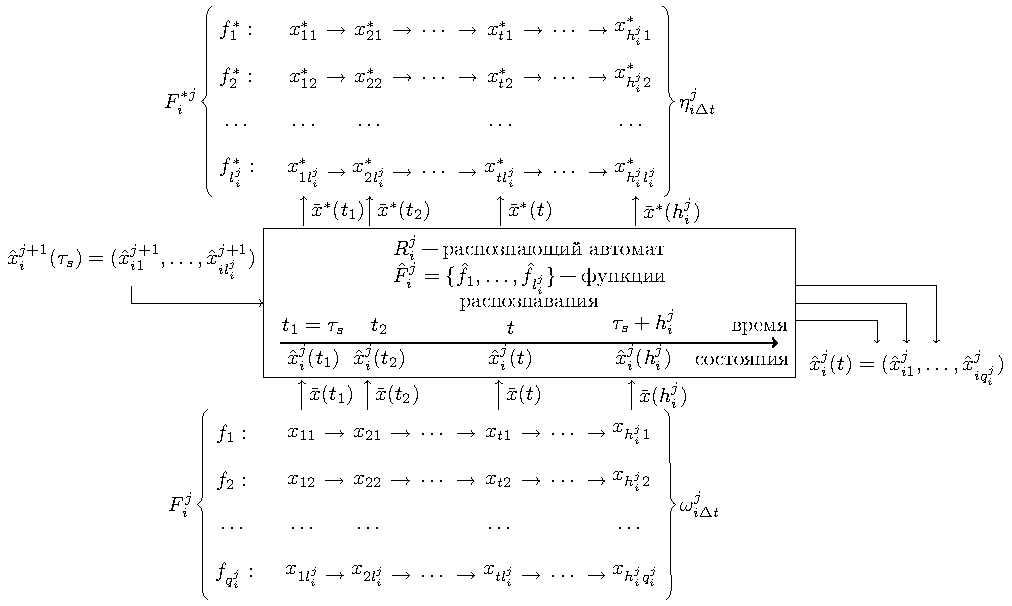
\includegraphics[width=1.0\linewidth]{rb_io}
		\caption{Вход и выход распознающего автомата $R_i^j$.}
		\label{fig:rb_io}
	\end{figure}
	
	\subsection{Процедурные и объектные признаки}
		Для определения компонент знака через описанный в предыдущем разделе $R$-автомат необходимо ввести ряд вспомогательных понятий. 
		
		Введём семейство бинарных отношений $\{\sqsubset,\sqsubset^1,\sqsubset^2,\dots\}$, определённых на декартовом произведении $\mathcal F\times \mathcal F$. Будем считать, что <<признак $f_1$ является составляющим признака $f_2$>> или <<признак $f_2$ измеряется по признаку $f_1$>> ($(f_1,f_2 )\in\sqsubset$ или $f_1\sqsubset f_2$) в том случае, если $f_1\dashv R_1^j, f_2\dashv R_2^{j+1}$, $R_2^{j+1}$ "--- родительский блок по отношению к $R_1^j$ и в множестве матриц предсказания $\mathcal Z_2$ признака $f_2$ существует как минимум одна матрица $Z_r^2$, содержащая некоторый столбец $\bar z_u^r$ с элементом $z_{uv}^r\not=0$, где $v$ "--- индекс признака $f_1$ во входном векторе для распознающего блока $R_2^{j+1}$.
		
		Пара признаков $(f_1,f_2)\in\sqsubset^t$ или $f_1\sqsubset^t f_2$, где $t\in\{1,2,\dots\}$, в~том случае, если $f_1\dashv R_1^j, f_2\dashv R_2^{j+1}$, $R_2^{j+1}$ "--- родительский блок по отношению к $R_1^j$ и в множестве матриц предсказания $\mathcal Z_2$ признака $f_2$ существует как минимум одна матрица $Z_r^2$, содержащая $t$–ый столбец $\bar z_t^r$ с~элементом $z_{tv}^r\not=0$, где $v$ "--- индекс признака $f_1$ во~входном векторе для распознающего блока $R_2^{j+1}$.
		
		Каждый элемент векторов"--~столбцов соотносится с~признаком из~входного множества признаков распознающего блока, что означает задание типа для каждого элемента вектора"--~столбца. Будем обозначать тип $k$-го элемента вектора-столбца распознающего блока $R_i^j$ как $f_i^j(k)\in F_i^j$, $k\in(1,q_i^j)$. 
		
		Введём два выделенных признака: $f_c$ является меткой условия, а $f_e$ "--- меткой эффекта. Пусть некоторый $R$-автомат, например $R_0^1$, распознаёт оба этих признака: $F_0^{*1}=\{f_c,f_e\}$. Признаки, которые распознаются распознающими блоками, выступающими родительскими по отношению к блоку $R_0^1$, будем называть процедурными признаками, остальные "--- объектными признаками. Это означает, что всё множество признаков делится на два подмножества: $\mathcal F=\mathcal F^{proc}\cup\mathcal F^{obj}$ и $\mathcal F^{proc}\cap\mathcal F^{obj}=\varnothing$.
		
		Для любого процедурного признака выполняются следующие естественные условия:
		\begin{itemize}
			\item условие всегда предшествует эффекту,
			\item условие всегда влечёт за собой эффект и
			\item все условия всегда отделены от своих эффектов.
		\end{itemize}
		
		Иными словами, если $f_1$ "--- процедурный признак, то если в столбце $\bar z_u^r$ матрицы предсказания $Z_r^1$ элемент $z_{uv}^r$, соответствующий признаку $f_c$, не равен $0$, то в этом столбце соответствующий признаку $f_e$ элемент вектора "--- нулевой, в столбце $z_{u+t}^r, t>0$. Наоборот "--- элемент $z_{u+t,v}^r$, соответствующий признаку $f_c$, равен $0$, а соответствующий признаку $f_e$ элемент "--- не нулевой. Столбцы матрицы предсказания $Z$, в которых соответствующий признаку $f_e$ элемент вектора не нулевой, будем называть \textit{столбцами эффектов}, а столбцы матрицы предсказания $Z$, в которых не равен нулю элемент вектора, соответствующий признаку $f_c$ "--- \textit{столбцами условий}. 
		
		Пополним семейство отношений $\{\sqsubset,\sqsubset^1,\sqsubset^2,\dots\}$ двумя отношениями: $\sqsubset^c$ и $\sqsubset^e$, принадлежность к~которым пары признаков $(f_1,f_2)$ свидетельствует о~том, что признак $f_1$ присутствует соответственно в~столбце условий и эффектов как минимум в~одной матрице предсказания процедурного признака $f_2$.
		
		\subsection{Определение компонент знака}
		При образовании нового знака $s$ до того, как формируемая тройка компонент получит имя, будем считать, что будущему знаку $s$ \textit{соответствует} некоторый признак $f(s)\in\mathcal F$, обладающий перцептом $\tilde p$, функциональным значением $\tilde m$ и биологическим смыслом $\tilde a$, которые после завершения процесса формирования знака $s$ становятся, соответственно, образом $p$, значением $m$ и личностным смыслом $a$.
		
		\begin{Def}
			Если $f_1$ "--- признак, соответствующий знаку $s_1$, то подмножество $\tilde p(f_1)$ множества $\mathcal F$ таких признаков, что $\forall f_i\in\tilde p(f_1) f_i\sqsubset f_1$, будем называть перцептом признака $f_1$.
		\end{Def}
		
		На множестве всех перцептов $\tilde P$ введём метрику $\rho_p(\tilde p(f_1),\tilde p(f_2))$, вычисляемую по~следующему правилу:
		\begin{itemize}
			\item если $f_1$ и $f_2$ распознаются разными распознающими блоками, т.~е. $f_1\dashv R_1^j, f_2\dashv R_2^i$, то $\rho_p(\tilde p(f_1),\tilde p(f_2))=\infty$,
			\item если $f_1$ и $f_2$ распознаются одним и тем~же распознающим блоком $R_1^j$ со~множеством входных признаков $F_1^j$ мощности $q$ и характерным временем $h$, то
			\begin{equation}
				\rho_p(\tilde p(f_1),\tilde p(f_2))=\min\limits_{\substack{Z_r^1\in Z_1\\Z_s^2\in Z_2}}\frac{1}{q\cdot h}\sum\limits_{u=1}^h\|\bar z_u^r-\bar z_u^s\|.
			\end{equation} 
		\end{itemize}
		
		\begin{Def}
			Если $f_1$ "--- признак, соответствующий знаку $s_1$, $f_2$ "--- процедурный признак, $f_1\sqsubset^c f_2$, то будем называть $f_2$ функциональным значением признака $f_1$. Множество всех функциональных значений признака $f_1$ будем обозначать $\tilde m(f_1)$.
		\end{Def}
		
		На множестве всех функциональных значений $\tilde M$ введём метрику $\rho_m(\tilde m(f_1),\tilde m(f_2))$, вычисляемую по следующему правилу:
		\begin{equation}
			\rho_m(\tilde m_1(f_1),\tilde m_2(f_2 ))=\min\limits_{\substack{f_i\in\tilde m(f_1 )\\f_j\in\tilde m(f_2 )}}\rho_p(\tilde p(f_i ),\tilde p(f_j )).
		\end{equation}
		
	\subsection{Семантический уровень обобщения} Определение ролевой структуры для алгоритма планирования.
	
	\noindent\colorbox{yellow}{
		\parbox{\dimexpr\linewidth-2\fboxsep}{Здесь я бы предложил дать определение типам обобщения на семантическом уровне.}
	}
	
	\section{Связывание образа и значения}
		В целях дальнейшего изложения рассмотрим подробнее строение матрицы предсказания процедурного признака. Матрицу предсказания $Z_r^p$ процедурного признака $f_p$ всегда можно представить в следующем виде:
		\begin{equation}
		Z_r^p=(\bar z_1^{r,c},\dots,\bar z_{j_1}^{r,c},\bar z_{j_{1+1}}^{r,e},\dots,\bar z_{i_1}^{r,e},\dots,\dots,\bar z_{i_{k-1}+1}^{r,c},\dots,\bar z_{j_k}^{r,c},\bar z_{j_k+1}^{r,e},\dots,\bar z_{i_k}^{r,e}),
		\end{equation}
		где $\bar z_j^{r,c}$ "--- столбцы условий, $\bar z_i^{r,e}$ "--- столбцы эффектов. 
		
		Величину $k$ будем называть сложностью процедурного признака. В~дальнейшем будем рассматривать простые матрицы предсказаний $k$-сложного процедурного признака:
		\begin{equation}
		Z_r^p=(\bar z_1^{r,c},\bar z_2^{r,e},\dots,\dots,\bar z_{2\cdot k-1}^{r,c},\bar z_{2\cdot k}^{r,e}).
		\end{equation}
		Краткая форма $k$-сложного процедурного признака $f_p$ имеет матрицу предсказания, в которой оставлены только первый столбец условий и последний столбец эффектов.
		
		Любой односложный, или элементарный, процедурный признак $f_p$, распознаваемый блоком $R_i^j$, можно представить в виде правила $r_p=(F_C(f_p),F_A(f_p),F_D(f_p))$, в котором:
		\begin{itemize}
			\item $F_C (f_p )\subseteq F_i^j$ "--- множество признаков "--- условий правила: $\forall f\in F_C(f_p)$ $f\sqsubset^c f_p$;
			\item $F_A(f_p)\subseteq F_i^j$ "--- множество добавляемых правилом признаков: $\forall f\in F_A(f_p)$ $f\sqsubset^e f_p,f\notin F_C$;
			\item $F_D(f_p)\subseteq F_i^j$ "--- множество удаляемых правилом признаков: $\forall f\in F_D(f_p)$ $f\notin F_A,f\in F_C$.
		\end{itemize}
		Очевидно, выполняются следующие соотношения: $F_A(f_p)\cap F_D(f_p)=\varnothing, F_A(f_p)\cap F_C(f_p)=\varnothing, F_D(f_p)\subseteq F_C(f_p)$.
		
		Таким образом, функциональное значение признака, а значит и значение знака, может быть задано правилом с определёнными множествами фактов условий и эффектов.
		\begin{Def}
			Процедурный признак $f_p^1$ c матрицей предсказания $Z=(\bar z_1^c,\bar z_2^e)$ выполняется на векторе $z$ длины $q$, если $z\cdot \bar z_1^c=\bar z_1^c$.
		\end{Def}
		Будем говорить, что процедурный признак $f_p^1$ выполним в~условиях процедурного признака $f_p^2$, если 
		\begin{itemize}
			\item оба признака распознаются одним и тем~же распознающим блоком $R_i^j$ и признак  $f_p^1$ выполняется на~столбце условий матрицы предсказания признака $f_p^2$,
			\item $f_p^1\dashv R_1^{j_1}, f_p^2\dashv R_2^{j_2}$, множества $F_C(f_p^1 )$ и $F_C(f_p^2)$ состоят из~одних и тех~же признаков, образуемый вектор $\tilde z$ (той же мощности, что и множество $F_1^{j_1}$) элементы которого, соответствующие признакам из $F_C(f_p^2)$ принимаются равными $1$,  остальные "--- $0$, и признак $f_p^1$ выполним на~векторе $\tilde z$. 
		\end{itemize}
		
		\begin{Def}
			Будем говорить, что два процедурных признака $f_p^1$ и $f_p^2$ конфликтуют, если выполнено по крайней мере одно из~следующих условий:
			\begin{itemize}
				\item $F_D(f_p^1)\cap F_A(f_p^2)\not=\varnothing$,
				\item $F_D(f_p^2)\cap F_A(f_p^1)\not=\varnothing$,
				\item $F_D(f_p^1)\cap F_C(f_p^2)\not=\varnothing$,
				\item $F_D(f_p^2)\cap F_C(f_p^1)\not=\varnothing$.
			\end{itemize}
		\end{Def}
		
		\begin{Def}
			Результатом операции сохраняющего приведения вектор"--~столбца $\bar z_1$ к~множеству входных признаков $F_{i_2}^{j_2}$ будем называть такой вектор $\bar z_3$ длины $q_{i_2}^{j_2}$, элемент которого $z_{3k}=1$, если $f_{i_1}^{j_1}(k)=f_{i_2}^{j_2}(k)$ и $z_{1k}=1$, иначе $z_{3k}=0$, и обозначать $(\bar z_1\rightarrow F_{i_2}^{j_2})=\bar z_3$.
		\end{Def}
		
		\begin{Def}
			Результатом операции сужающего приведения вектор"--~столбца $\bar z_1$ к~некоторому столбцу $\bar z_2$ распознающего блока $R_{i_2}^{j_2}$ будем называть такой вектор $\bar z_3$ длины $q_{i_2}^{j_2}$, элемент которого $z_{3k}=1$, если $f_{i_1}^{j_1}(k)=f_{i_2}^{j_2}(k)$, $z_{2k}=1$ и $z_{1k}=1$, иначе $z_{3k}=0$, и обозначать $(\bar z_1\Rightarrow \bar z_2)=\bar z_3$.
		\end{Def}
		
		Будем считать, что у субъекта имеется опыт наблюдения, который выражается в виде отношения $\Psi_p^m: \Psi_p^m(\tilde p)=\tilde m$, в том случае, если $\tilde p\in\tilde P$ является перцептом некоторого признака $f$, а $\tilde m\in\tilde M$ "--- функциональным значением того же признака $f$.
		
		Ниже представлен алгоритм доопределения функции $\Psi_p^m$, который и отражает собой суть итерационного процесса во время образования знака согласно алгоритму из первой части статьи. Доопределение проводится на~новую пару $(\tilde p,\tilde m)$, где функциональное значение $\tilde m$ строится в сравнении с эталоном $\tilde m^0$, а перцепт $\tilde p$ формируется на основе подмножества составляющих признаков $\hat F$. Доопределение функции $\Psi_p^m$ означает формирование нового признака $f^*$, т.~е. его первой матрицы предсказания $Z^*$ в~рамках распознающего блока $R^*$.
				
	\begin{algorithm}
		\caption{Алгоритм $\mathfrak{A}_{pm}$}\label{alg:pm}
		\begin{algorithmic}[1]
				\Require $\tilde m^0=\{f_p\}, \Psi_p^m, \hat F\subseteq \mathcal F$;
	
	\State $\tilde p^{*(0)} := \varnothing$;
	\State $Z^{*(0)} := \varnothing$;
	\State $t := 0$;
	
	\ForAll{$f^{(t)}\in \hat F$}
		\If{$\exists \tilde m^{(t)}\in \tilde M$ такое, что $(\tilde p(f^{(t)}),\tilde m^{(t)})\in\Psi_p^m$, $\tilde m^{(t)}$ выполним в условиях признака $f_p$, $\nexists f: f\in\tilde p^{*(t)},(\tilde p(f),\tilde m(f))\in\Psi_p^m, \tilde m^0$ конфликтует с $\tilde m^{(t)}$}
			\State $\tilde p^{*(t)}=\tilde p^{*(t)}\cup\{f^{(t)}\}$;
	
			\If{$\exists R_i^j$ такой, что $f^{(t)}\in F_i^j$}
				\State $R_i^{j(t)}:=R_i^j$;
			\Else
				\State $R_i^{j(t)}:=\argmax\limits_{\mathcal R} (F_i^j\cap\tilde p^{(t)}), F_i^{j(t)}:=F_i^{j(t)}\cup f^{(t)}$;
			\EndIf
	
			\State $\bar z_s:=(z_{s1},z_{s2},\dots,z_{sq}), z_{sk}=1$, если $k$ -- индекс признака $f^{(t)}$ во входном векторе распознающего блока $R_i^{j(t)}$ и $z_{sk}=0$ иначе;
			\State $Z^{*(t)}:=Z^{*(t)}\cup\bar z_s$;
			\State $Z_p^{(t)}:=(\bar z_1^{c(t)},\bar z_2^{e(t)},\dots,\bar z_{2\cdot k-1}^{c(t)},\bar z_{2\cdot k}^{e(t)})$, где $\bar z_i^{c(t)}=\bigvee\limits_{\tilde m_j^{(t)}}(\bar z_j^{c(t)}\rightarrow F_p^j),$ 
	\\\hspace{3.0cm}$\bar z_i^{e(t)}=\bigvee\limits_{\tilde m_j^{(t)}}(\bar z_j^{e(t)}\Rightarrow\bar z_j^e)$;
		\EndIf
	
		\State $\tilde m^{*(t)}=\{f_p^{(t)}\}$;
		\State $\mathcal Z^{*(t)}=\{Z^{*(t)}\}$;
		\State $t=t+1$;
	\EndFor
	
	\Return $\Psi_p^m$, определённая на паре $(\tilde p, \tilde m)$, где $\tilde p=\tilde p^{*(|\hat F|)}$, $\tilde m=\tilde m^{*(|\hat F|)}$, $f^*, Z^*=Z^{*(|\hat F|)},\mathcal Z^*=\{Z^*\}$;
		\end{algorithmic}			
	\end{algorithm}
	
	\begin{Theorem}[о корректности алгоритма $\mathfrak A_{pm}$]
		Алгоритм $\mathfrak A_{pm}$ корректен, т.~е. последовательность функциональных значений $\langle\tilde m^{*(0)},\tilde m^{*(1)},\dots\rangle$, которая строится с помощью алгоритма $\mathfrak A_{pm}$ для функционального значения $\tilde m^0$, сходится к $\tilde m^0$.
	\end{Theorem}
	
	\begin{Proof}
		Рассмотрим два элемента последовательности $\tilde m^{*(t)}=\{f_p^{(t)}\}$ и $\tilde m^{*(t+1)}=\{f_p^{(t+1)}\}$. Соответствующие матрицы предсказания будут иметь следующий вид:
		\begin{eqnarray}
		Z_p^{(t)}=(\bar z_1^{c(t)},\bar z_2^{e(t)},\dots,\dots,\bar z_{2\cdot k-1}^{c(t)},\bar z_{2\cdot k}^{e(t)}),\\
		Z_p^{(t+1)}=(\bar z_1^{c(t+1)},\bar z_2^{e(t+1)},\dots,\dots,\bar z_{2\cdot k-1}^{c(t+1)},\bar z_{2\cdot k}^{e(t+1)}).
		\end{eqnarray}
		Если на шаге 1 и 2 алгоритма $\mathfrak A_{pm}$ на $(t+1)$-й итерации не был найден подходящий признак, то матрицы $Z_p^{(t)}$ и $Z_p^{(t+1)}$ равны. Рассмотрим случай, когда был найден подходящий признак $f^{(t+1)}$ с функциональным значением $\tilde m^{(t+1)}=\{\tilde f_p^{(t+1)}\}$ с соответствующей матрицей предсказания $\tilde Z_p^{(t+1)}=(\bar z^{c(t+1)},\bar z^{e(t+1)})$.
		
		Т.~к. выполнено условие шага 1, то признак $\tilde f_p^{(t+1)}$ выполним на некотором $(2\cdot s-1$-м столбце условий матрицы предсказания признака $f_p$. Это означает, что матрицы $Z_p^{(t)}$ и $Z_p^{(t+1)}$ будут отличать только в двух вектор-столбцах $(2\cdot s-1)$-м и $(2\cdot s)$-м:
		\begin{equation}
		\bar z_{2\cdot s-1}^{c(t+1)}=\bar z_{2\cdot s-1}^{c(t)}\vee (\bar z^{c(t+1)}\rightarrow F_p^j),\bar z_{2\cdot s}^{e(t+1)}=\bar z_{2\cdot s}^{e(t)}\vee(\bar z^{e(t+1)}\Rightarrow \bar z_{2\cdot s}^e).
		\end{equation}
		По определению расстояние между функциональными значениями $\tilde m^{(t)}$ и $\tilde m^0$ примет следующее значение:
		\begin{eqnarray}
		\rho_m(\tilde m^{(t)},\tilde m^0)=\min\limits_{\substack{f_i\in\tilde m^{(t)}\\f_j\in\tilde m^0}}\rho_p(\tilde p(f_i),\tilde p(f_j ))=\rho_p(\tilde p(f_p^{(t)}),\tilde p(f_p))=\nonumber \\
		=\frac{1}{q\cdot h}\sum\limits_{\substack{\bar z_u^1\in Z_p^{(t)}\\\bar z_u^2\in Z_p}}\|\bar z_u^1-\bar z_u^2\|.
		\end{eqnarray}
		Аналогично для $\tilde m^{(t+1)}$:
		\begin{equation}
		\rho_m(\tilde m^{(t+1)},\tilde m^0)=\frac{1}{q\cdot h}\sum_{\substack{\bar z_u^1\in Z_p^{(t+1)}\\\bar z_u^2\in Z_p}}\|\bar z_u^1-\bar z_u^2\|.
		\end{equation}
		Рассмотрим разность 
		\begin{eqnarray}
		\rho_m(\tilde m^{(t)},\tilde m^0)-\rho_m(\tilde m^{(t+1)},\tilde m^0)=\frac{1}{q\cdot h}(\|\bar z_{2\cdot s-1}^{c(t)}-\bar z_{2\cdot s-1}^c\|+\|\bar z_{2\cdot s}^{e(t)}-\bar z_{2\cdot s}^e\|-\nonumber \\
		-\|\bar z_{2\cdot s-1}^{c(t+1)}-\bar z_{2\cdot s-1}^c\|-\|\bar z_{2\cdot s}^{e(t+1)}-\bar z_{2\cdot s}^e\|)=\frac{1}{q\cdot h}(\|\bar z_{2\cdot s-1}^{c(t)}-\bar z_{2\cdot s-1}^c\|+\nonumber \\
		+\|\bar z_{2\cdot s}^{e(t)}-\bar z_{2\cdot s}^e\|-\|\bar z_{2\cdot s-1}^{c(t)}\vee(\bar z^{c(t+1)}\rightarrow F_p^j)-\bar z_{2\cdot s-1}^c\|-\nonumber \\
		-\|\bar z_{2\cdot s}^{e(t)}\vee(\bar z^{e(t+1)}\Rightarrow\bar z_{2\cdot s}^e)-\bar z_{2\cdot s}^e\|),
		\end{eqnarray}
		где $\bar z_{2\cdot s-1}^c,\bar z_{2\cdot s}^e$ "--- столбцы матрицы предсказания процедурного признака $f_p$, соответствующего функциональному значению $\tilde m^0$.
		
		Так как $\tilde f_p^{(t+1)}$ выполним на $(2\cdot s-1)$–м столбце условий матрицы предсказания признака $f_p$, то после применении операции приведения $\bar z^{c(t+1)}\rightarrow F_p^j$ в результирующем векторе единицы появляются только на тех же местах что и в векторе $\bar z_{2\cdot s-1}^c$. 
		
		Это означает, что в векторе $\bar z_{2\cdot s-1}^{c(t)}\vee(\bar z^{c(t+1)}\rightarrow F_p^j)$ по сравнению с вектором $\bar z_{2\cdot s-1}^{c(t)}$  единицы находятся только в тех же местах, что и в векторе $\bar z_{2\cdot s-1}^c$, а новых нулей не появляется. В следствие чего разность $\|\bar z_{2\cdot s-1}^{c(t)}-\bar z_{2\cdot s-1}^c\|-\|\bar z_{2\cdot s-1}^{c(t)}\vee(\bar z^{c(t+1)}\rightarrow F_p^j)-\bar z_{2\cdot s-1}^c\|$ всегда больше нуля.
		
		Так как для столбцов эффектов применяется операция сужающего приведения, которая оставляет единицы только на тех местах, на которых одновременно находятся единицы в приводимом векторе и векторе, к которому осуществляется приведение. В связи с этим разность $\|\bar z_{2\cdot s}^{e(t)}-\bar z_{2\cdot s}^e\|-\|\bar z_{2\cdot s}^{e(t)}\vee(\bar z^{e(t+1)}\Rightarrow\bar z_{2\cdot s}^e)-\bar z_{2\cdot s}^e\|$ также больше нуля.
		
		Так как обе разности в скобках выражения для $\rho_m(\tilde m^{(t)},\tilde m^0)-\rho_m(\tilde m^{(t+1)},\tilde m^0)$ больше нуля, то отсюда следует, что функциональное значение $\tilde m^{(t+1)}$ ближе к $\tilde m^0$. В виду произвольности выбора итерации $t$, это приводит к сходимости всей последовательности $\langle\tilde m^{*(0)},\tilde m^{*(1)},\dots\rangle$. 
	\end{Proof}
	
	\section{Самосознание и его функции} .
	
	\noindent\colorbox{yellow}{
		\parbox{\dimexpr\linewidth-2\fboxsep}{Здесь я бы предложил дать психологическое описание строения и функций самосознания.}
	}
	
	\section{Алгоритм планирования}	.

	\noindent\colorbox{yellow}{
		\parbox{\dimexpr\linewidth-2\fboxsep}{Описание и определение функций оценки $\Phi_a$ и $\Phi_p$.}
	}

	Планом $Plan$ будем называть такую последовательность личностных смыслов, в которой действие, представляемое очередным личностным смыслом не конфликтует с предыдущим в цепочке действием.
	
	Целевая ситуация строится исходя из образа процедурного признака, связанного с личностным смыслом, который был определён в процессе целеполагания для целевого знака (см. первую часть статьи).
	
	На странице \pageref{alg:beh_plan} представлен алгоритм планирования поведения.
	\begin{algorithm}
		\caption{Алгоритм $\mathfrak{A}_{bp}$}\label{alg:beh_plan}
		\begin{algorithmic}[1]
				\Require начальная ситуация $S_{st}$, целевая ситуация $S_{goal}$, включающая в себя знак мотива $s_{goal}$, функции оценки $\Phi_a$ и $\Phi_p$;
	\Ensure план $Plan$;
	\algrule
	\State $F_{st}^{obj}=\varnothing$; \Comment{множество объектных признаков начальной ситуации}
	\ForAll $s\in S_{st}$
		\If{$f(s)\in\mathcal F^{obj}$}
			\State $F_{st}^{obj}= F_{st}^{obj}\cup\{f(s)\}$; 
		\EndIf
	\EndFor
	
	\State $Plan=\Call{Planning}{\varnothing,S_{goal}}$;
	
	\Function{Planning}{$Plan, S_{cur}$}
		\State $F_{cur}=\bigcup\limits_{s\in S_{cur}}\{f(s)\}$; \Comment{множество признаков текущей ситуации планирования}
		\State $F_{st}=\bigcup\limits_{s\in S_{st}}\{f(s)\}$; \Comment{множество признаков начальной ситуации}
		\State $M_{st}=\bigcup\limits_{f\in F_{st}}m(f)$;
		\State $\Delta=F_{st}\setminus F_{cur}$; \Comment{текущая невязка состояний}
		
		\State $M_{forw}\subseteq M_{st}:\begin{cases}
			|\bigcup\limits_{\mu\in M_{forw}}F_A(\mu)\setminus\Delta|\rightarrow\max,\\
			|\bigcap\limits_{\mu\in M_{forw}}F_A(\mu)\setminus\Delta|\rightarrow\min;
		\end{cases}$ \Comment{Решение minmax задачи}
		
		\ForAll $\mu_j\in M_{forw}$
			\If{$\exists \mu_k\in M_{forw}$ такой, что $\mu_k\not =\mu_i$ и $\mu_k$ конфликтует с $\mu_j$}
				\State $\mu_{del}=\argmin\limits_{\mu\in\{\mu_k,\mu_j\}}|F_A(\mu)\setminus\Delta|$;
				\State $M_{forw}= M_{forw}\setminus\{\mu_{del}\}$; \Comment{Удаляем конфликтующие признаки}
			\EndIf
		\EndFor
		
		\State $A_{forw} = \bigcup\limits_{\mu\in M_{forw}}\{\Call{Interior}{\mu}\}$; \Comment{текущее множестов личностных смыслов}
		\State $\tilde A_{forw}=\Phi_a(A_{forw},f_{goal})$; \Comment{выбор предпочитаемых действий}
		\If{$\bigcup\limits_{a\in \tilde A_{forw}}F_C(a)\subseteq F_{st}$ и $F_{cur}\subseteq F_{st}\cup\bigcup\limits_{a\in \tilde A_{forw}}F_C(a)\setminus\bigcup\limits_{a\in \tilde A_{forw}}F_D(a)$}
			\State \Return $Plan\cup{\tilde A_{forw}}$;		\Comment{возвращаем обновленный план}
		\Else
			\State $\Delta^* = \Phi_p(\Delta, f_{goal})$; \Comment{Ранжирование критических признаков}
			\State $\tilde F_a^{back} = \varnothing$; 
			\ForAll $f_k\in\Delta^*$ 
				\State $m_k = \tilde m(f_k)$; \Comment{определение значение $k$-го знака}
				\State $F_a^{back} = \varnothing$;
				\ForAll $f_p\in m_k$
					\State $F_a^{back}=F_a^{back}\cup\{\Call{Interior}{f_p}\}$;
				\EndFor 
				\State $\tilde F_a^{back}=\tilde F_a^{back}\cup\Phi_a(F_a^{back}, f_{goal})$; \Comment{выбор предпочитаемых действий}
			\EndFor
			
			\ForAll $f_j\in \tilde F_a^{back}$
				\If{$\exists f_k\in \tilde F_a^{back}$ такой, что $f_k\not =f_i$ и $f_k$ конфликтует с $f_j$}
					\State $\tilde F_a^{back} = \tilde F_a^{back}\setminus\{f_k\}$; \Comment{Удаляем конфликтующие признаки}
				\EndIf
			\EndFor
			
			
			\If{$\Delta\not\subseteq\bigcup\limits_{f\in\tilde F_a^{back}}F_A(f)$}
				\State\Return невозможно построить план;
			\Else
				\State \Return \Call{Planning}{$Plan, \bigcup\limits_{f\in F_a^{back}}F_C(f)$};						
			\EndIf
		\EndIf

	\EndFunction
		\end{algorithmic}
	\end{algorithm}
	
	\section*{Заключение} Подведение общих итогов.
	
	\noindent\colorbox{yellow}{
		\parbox{\dimexpr\linewidth-2\fboxsep}{Про архитектуру агентов и распределение ролей.}
	}
	
	\titleformat{\section}{\normalfont\centering\MakeUppercase}{\thesection.}{1pt}{}[]
	
	%	\nocite{*}
	\inputencoding{cp1251}
	\bibliography{../../biblio/main}
	\inputencoding{utf8}
\end{document}